\chapter{Datenformate}

Grundsätzlich unterscheidet man zwischen binären und strukturierten Formaten. Binäre Formate vereinbaren die Struktur der zu übertragenden Daten im Vorhinein und übertragen anschließend einen Binärdatenstrom. Strukturierte Verfahren hingegen übertragen die Struktur der Daten bei jeder Übertragung mit. Diese Formate basieren meist auf einem Textformat und sind daher wesentlich leicher zu debuggen. Dieser Vorteil wird jedoch mit einer erhöhten zu übertragenden Datenmenge erkauft.


\section{Strukturierte Datenformate}

JSON (JavaScript Object Notation), XML (Extensible Markup Language) und YAML (YAML Ain't Markup Language) sind führende Datenformate, die für den strukturierten Datenaustausch über das Internet entwickelt wurden. JSON, entstanden aus der JavaScript-Programmiersprache, wird seit den frühen 2000er Jahren hauptsächlich für den Datenaustausch zwischen Servern und Webanwendungen sowie in Konfigurationsdateien und NoSQL-Datenbanken wie MongoDB verwendet. Es ist effizienter und einfacher zu handhaben als XML, welches seit den späten 1990er Jahren von W3C standardisiert wurde und sich durch eine strenge, erweiterbare Struktur auszeichnet, ideal für komplexe Anwendungen wie Unternehmenssoftware. YAML, eingeführt im Jahr 2001, bietet eine menschenlesbare Struktur, die in Konfigurationsdateien weit verbreitet ist und eine klare, effiziente Organisation von Daten ermöglicht.

\begin{figure}[h]
	\centering
	\begin{minipage}{0.32\textwidth}
		\centering
		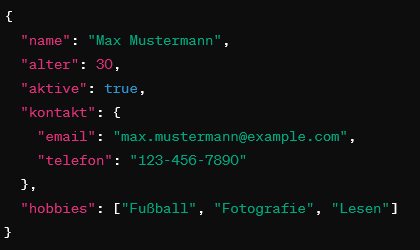
\includegraphics[width=\textwidth]{figures/jsonexample.png}
		\caption{JSON-Daten}
		\label{fig:json}
	\end{minipage}\hfill
	\begin{minipage}{0.32\textwidth}
		\centering
		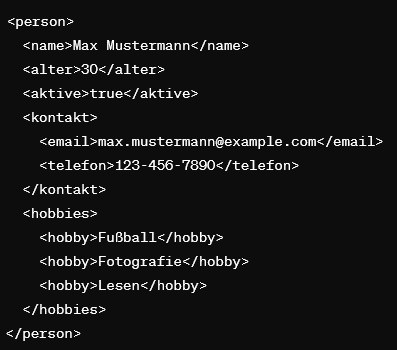
\includegraphics[width=\textwidth]{figures/xmlexample.png}
		\caption{XML-Daten}
		\label{fig:xml}
	\end{minipage}\hfill
	\begin{minipage}{0.32\textwidth}
		\centering
		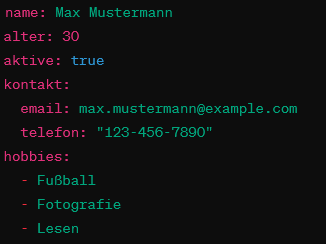
\includegraphics[width=\textwidth]{figures/ymlexample.png}
		\caption{YML-Daten}
		\label{fig:yaml}
	\end{minipage}
\end{figure}


\section{Binäre Datenformate}

Protocol Buffers (Protobuf), Cap'n Proto und Netcode for Game Objects (NfGO) sind wichtige binäre Datenformate für effiziente Datenübertragung in kritischen Anwendungsbereichen. Protobuf, von Google entwickelt, optimiert den Datenaustausch in verteilten Systemen und mobilen Anwendungen durch Codegenerierung aus .proto Dateien, bietet strikte Typsicherheit und Kompatibilität. Cap'n Proto, eine Weiterentwicklung von Protobuf, ermöglicht das Lesen von Daten ohne Umwandlung in eine Zwischenrepräsentation, wodurch die Leistung verbessert wird. NfGO, verwendet in Multiplayer-Videospielen, unterstützt synchronisierte Interaktionen durch effiziente Serialisierung und Differential Compression, um Netzwerkeffizienz und Spielerlebnis zu optimieren.

\begin{figure}[]
	\centering
	\begin{minipage}{0.48\textwidth}
		\centering
		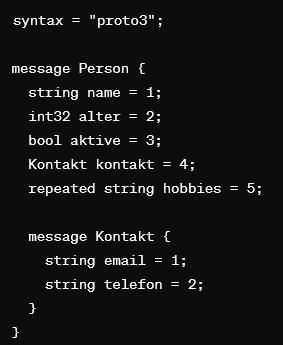
\includegraphics[width=\textwidth]{figures/protobufexample.png}
		\caption{Protobuf Datenstruktur}
		\label{fig:protobuf}
	\end{minipage}\hfill
	\begin{minipage}{0.48\textwidth}
		\centering
		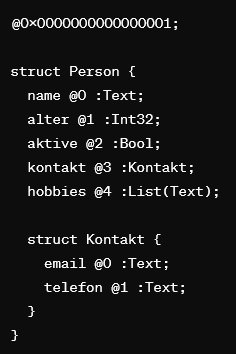
\includegraphics[width=\textwidth]{figures/capnprotoexample.png}
		\caption{Cap'n Proto Datenstruktur}
		\label{fig:capnproto}
	\end{minipage}\hfill
	
\end{figure}


\section{Serialisierung in Unity}

Unity bietet eine Reihe an Möglichkeiten an, mit denen Entwickler ihre Daten serialisieren können. Diese Methoden sind jedoch zu einem nicht unerheblichen Teil vollständig in das Unity-Universum integriert und können daher nicht außerhalb verwendet werden. Insgesamt sind für beide Projekte also einige Basiskonzepte vorhanden, die in beiden Projekten verwendet wurden.

\subsection{Byte-Arrays}

Ganz allgemein haben wir uns bei der Definition der Interfaces für die verschiedenen Aufgabenabschnitte darauf geeinigt, dass Objekte in Byte-Arrays zu serialisieren sind. Diese Byte-Arrays werden dann von der Netzwerkschnittstelle übertragen. Aus diesem Grund zielt die Umsetzung in beiden Projekten darauf ab, C\#-Klassen in Byte-Arrays zu übersetzen und zurück.
